\begin{figure}[ht]
	\centering
	\footnotesize

	\psfrag{x}[l][l] {$x$}
	\psfrag{x1}[l][l] {$x_1$}
	\psfrag{x2}[l][l] {$x_2$}

	\psfrag{r}[l][l] {$\rho(x,t)$}
	\psfrag{r1}[l][l] {$\rho(x_{1},t)$}
	\psfrag{r2}[l][l] {$\rho(x_{2},t)$}

	\psfrag{1}[c][c] {$T_{b} = ... $}
	\psfrag{2}[c][c] {$T_{b} = ... $}
	\psfrag{3}[c][c] {$T_{b} = ... $}
	\psfrag{4}[c][c] {$T_{b} = ... $}
	\psfrag{5}[c][c] {$T_{b} = ... $}
	\psfrag{6}[c][c] {$T_{b} = ... $}


	\psfrag{plc}[l][l] {$\textsc{Polycrystalline LLZO}$}

	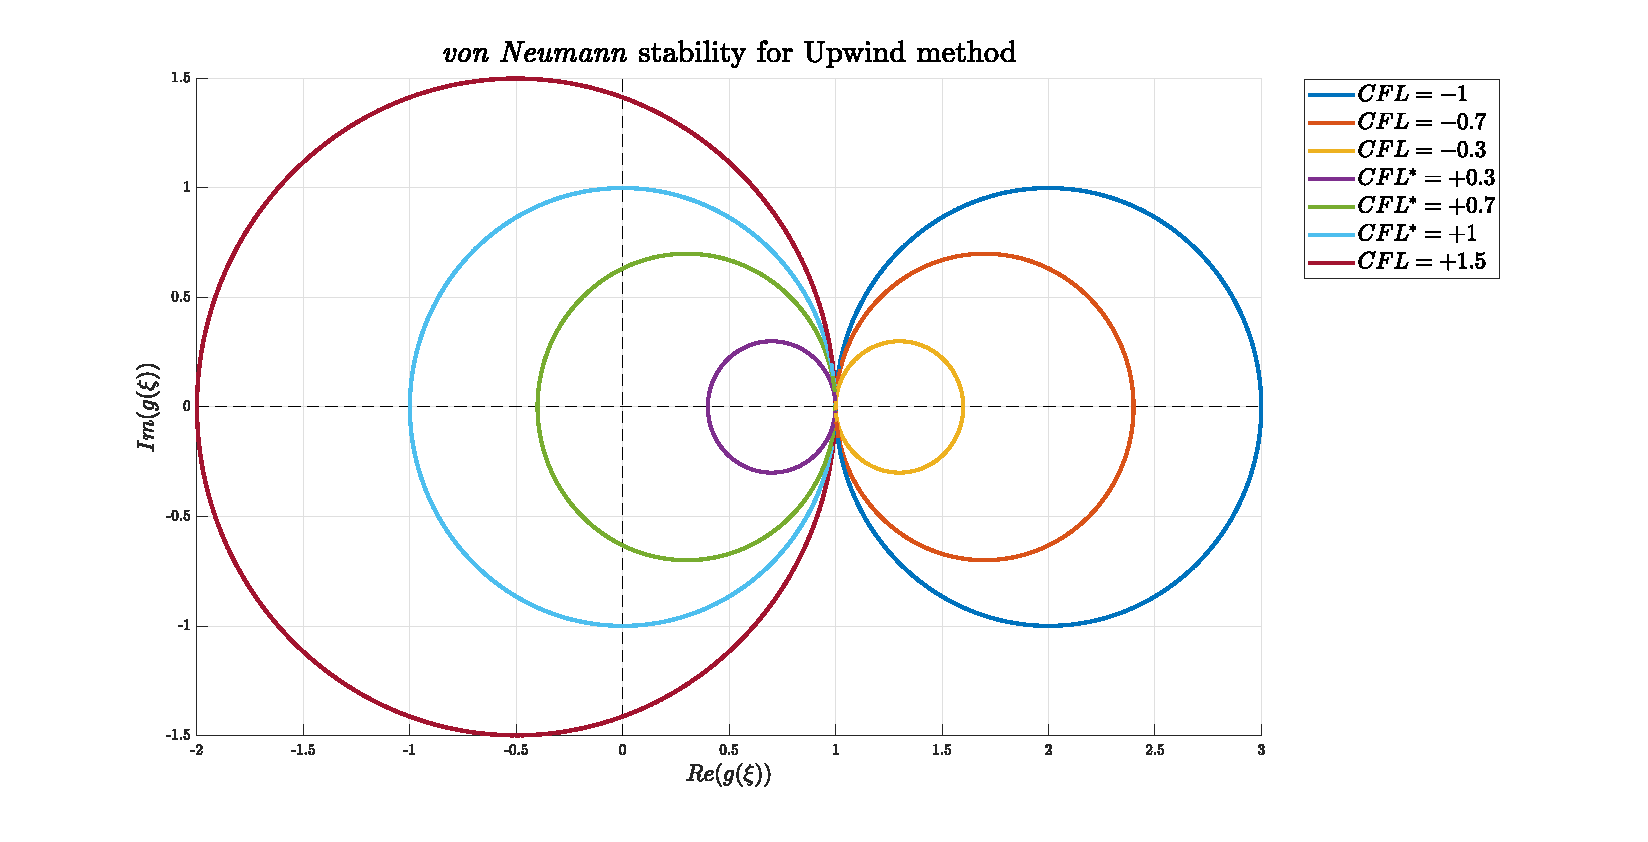
\includegraphics[width=1.0\textwidth]{vonNeumannstabil.eps}
	\caption{\emph{von Neumann} stability analysis for Upwind method.}
	\label{\LABEL}
\end{figure}
